\chapter*{Teori}

\begin{enumerate}
	\item 1.	File CSV (Comma Seperated Values)  merupakan format data pada basis data yang menggunakan tanda koma  dan titik koma untuk memisahkan setiap recordnya.  CSV ini digunakan pengguna untuk menginputkan data kedalam database secara sederhana.
    Contohnya :
	
	\begin{figure} [h]
	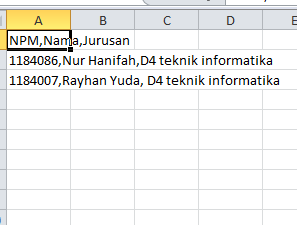
\includegraphics[width=5cm]{poto/poto.png}
	\centering
	\end{figure}		
	
	\item Aplikasi yang dapat membuat file CSV adalah Text editor( Notepad,Worpad, dan lain-lain), spreadsheet(Microsoft Excel,dll).
	
	\item Cara membuat dan membaca file CSV di excel:
	\begin{itemize}
	\item Buka Ms.Excell dan buat dokument baru
	\end{itemize}
	\begin{itemize}
	\item Lalu simpan data tersebut dengan mengklik "save as" dan ganti jenis filenya dengan format .csv
	\end{itemize}

	\item library csv(command Seperated Values) adalah format eksport dan import paling umum yang digunakan untuk spreadsheet dan basisdata.Modul CSV mengimplementasikan kelas untuk membaca dan menulis data tabular dalam format CSV.
	
	
	\item library Pandas digunakan sebagai  alat analisis data dan struktur untuk bahasa pemrograman Python. Dengan adanhya pandas kita dapat mengelola data dengan mudah salah satunya dengan fitur dataframe. Dengan adanuya dataframe ini kita dapat membaca sebuah file dan menjadikannya sebuah table serta juga dapat mengelola data dengan menggunkan operasi join,distinct, grup by,agrerasi, dan lain-lainnya yang terdapat pada SQL.


	\item Fungsi yang terdapat pada library CSV:\\
	\begin{itemize}
	\item Reade, Fungsi Reader diguunakan untuk membaca  isi file
	\begin{lstlisting}[language=Python]
import csv

with open('Book1.csv') as csv_file:
    csv_reader = csv.reader(csv_file , delimiter=',')
    for row in csv_reader:
        print(row)
\end{lstlisting}
	\end{itemize}
	\begin{itemize}
	\item Dict Reader, Fungsi Dict Reader digunakan untuk membaca isi file yang terdapat di dictionary
	\begin{lstlisting}[language=Python]
import csv

with open('Book1.csv',mode='r') as csv_file:
    csv_reader = csv.DictReader(csv_file)
    for row in csv_reader:
        print(row['NPM'], row['Nama'], row['Jurusan'])
\end{lstlisting}
	\end{itemize}
	\begin{itemize}
	\item Write, Fungsi Write ini digunakan untuk menulis file
	\begin{lstlisting}[language=Python]
import csv

with open('Jurusan1', mode='w') as csv_file:
     csv_writer = csv.writer(csv_file, delimiter=',', quotechar='"', quoting=csv.QUOTE_MINIMAL) 
     csv_writer.writerow(['NPM' , 'Nama' , 'Jurusan' ])
     csv_writer.writerow(['1184020' , 'Dudu' , 'TI' ])
     csv_writer.writerow(['1184030' , 'Didi' , 'LB' ])
\end{lstlisting}
	\end{itemize}
	\begin{itemize}
	\item Dict Write, Fungsi Dict Write digunakan untuk menulis file yang ada di dictionary
	\begin{lstlisting}[language=Python]
import csv

with open('Jurusan1', mode='w') as csv_file:
     fieldnames=['NPM','Nama']
     writer=csv.DictWriter(csv_file,fieldnames=fieldnames)

     writer.writeheader()
     writer.writerow({'NPM':'1184020' , 'Nama':'Dudu' })
     writer.writerow({'NPM':'1184030' , 'Nama':'Didi' })
\end{lstlisting}
	\end{itemize}
	
	\item Fungsi yang terdapat di libarary pandas
	\begin{itemize}
	\item to\_csv, untuk menulis file yang type nya CSV
	\begin{lstlisting}[language=Python]
import pandas

df=pandas.read_csv('Book1.csv')
df.to_csv('Book4.csv')

\end{lstlisting}
	\end{itemize}
	\begin{itemize}
	\item read\_csv, untuk membaca file type CSV
	\begin{lstlisting}[language=Python]
import pandas

df=pandas.read_csv('Book1.csv')
print(df)

\end{lstlisting}
	\end{itemize}
	
	
\end{enumerate}


